\documentclass[10pt]{article}

\usepackage[hmargin=0.76in,vmargin=0.62in]{geometry}
\usepackage[T1]{fontenc}
\usepackage{lmodern}
\usepackage{microtype}
\usepackage{amsmath,amssymb,amsthm,mathtools}
\usepackage{enumitem}
\usepackage{titlesec}
\usepackage{xcolor}
\usepackage{tikz}
\usetikzlibrary{arrows.meta}
\usepackage[hidelinks]{hyperref}

\setlength{\parindent}{0pt}
\setlength{\parskip}{2pt}
\setlength{\emergencystretch}{3em}
\setlength{\abovedisplayskip}{5pt}
\setlength{\belowdisplayskip}{5pt}
\setlength{\abovedisplayshortskip}{3pt}
\setlength{\belowdisplayshortskip}{3pt}
\setlist[enumerate]{leftmargin=1.45em,itemsep=1pt,topsep=2pt}
\titlespacing*{\section}{0pt}{7pt}{2pt}
\titlespacing*{\subsection}{0pt}{5pt}{1pt}
\titleformat{\section}{\large\bfseries}{}{0pt}{}
\titleformat{\subsection}{\normalsize\bfseries}{}{0pt}{}

\newtheorem{proposition}{Proposition}
\theoremstyle{definition}
\newtheorem{definition}{Definition}
\newtheorem{corollary}{Corollary}
\newcommand{\dd}{\mathrm d}

\definecolor{oldblue}{HTML}{2B5C88}
\definecolor{newred}{HTML}{B1433E}
\definecolor{midgray}{HTML}{666666}

\begin{document}

\begin{center}
{\LARGE\bfseries Housing Reallocation and Demographic Transitions}\par
\vspace{2pt}
{\large A two-generation model}\par
\end{center}

\section{Environment}

\textbf{Agents.} Time is discrete and one period is one generation. At date
$t$, the economy contains $Y_t$ young households and $O_t$ old households. A
young household has income $y_i$ and liquid wealth $b_i$, drawn from a fixed
type distribution $F$. A young renter becomes an old renter, a young owner
becomes an old incumbent, and every old household exits at the end of the
period.

\textbf{Preferences.} A young household values adult consumption $c$, space
net of children's needs, and completed fertility:
\begin{equation}
 u_t^Y(c,h,n)=\log c+\alpha\log(h-\kappa n)+\vartheta_t\log n.
 \label{eq:young_utility}
\end{equation}
Each child uses $\chi>0$ units of goods and $\kappa>0$ units of space. An old
household values consumption, retained housing, and the estate delivered at
death:
\begin{equation}
 u^O(c^O,h^O,e)=\log c^O+\gamma\log h^O+\omega_B\log e.
 \label{eq:old_utility}
\end{equation}
The financial sector supplies liquid claims and absorbs estates at price $q$.

\textbf{Housing and financial markets.} A fixed stock $\bar H$ produces one
unit of housing services per unit and period. Renters can occupy at most
$\bar h^R$, while owners can occupy at most $\bar h^O>\bar h^R$. The asset
price is $P_t$, one-period-ahead goods have price $q\in(0,1)$, and
$R=q^{-1}$. Competitive housing intermediaries imply the user-cost relation:
\begin{equation}
 r_t=(1+\tau_t^p)P_t-qP_{t+1},
 \label{eq:user_cost}
\end{equation}
where $\tau_t^pP_t$ is the recurring property tax per unit.

\textbf{Ownership and taxation.} A buyer finances the share $\phi$ of the
purchase with a one-period mortgage and posts $(1-\phi)P_th$ at closing. The
mortgage advance is $\phi P_th$ and its next-period repayment is
$R\phi P_th$. Selling a unit realizes the capital-gains tax
\begin{equation}
 \ell_t=\tau^g[P_t-P_{t-1}]_+,
 \label{eq:gains_tax}
\end{equation}
while a unit retained until death enters the estate with stepped-up basis. The
tax is zero whenever the real asset price is constant. These cash flows give
two tenure-specific costs. Buying a unit, paying its
property tax, and selling it next period costs:
\begin{equation}
 r_t^O=(1+\tau_t^p)P_t-q(P_{t+1}-\ell_{t+1})
 =r_t+q\ell_{t+1}.
 \label{eq:owner_user_cost}
\end{equation}
For an old incumbent, retaining a unit rather than selling it, paying the
property tax, and placing its next-period value in the estate costs:
\begin{equation}
 r_t^I=(P_t-\ell_t)+\tau_t^pP_t-qP_{t+1}=r_t-\ell_t.
 \label{eq:incumbent_user_cost}
\end{equation}
Thus the buyer anticipates the future tax, while the incumbent avoids the
current tax by retaining the house.

\textbf{Demography.} Each child generates $\nu>0$ future young households
after survival and household formation. The children of a household affect
future cohort size but do not inherit that household's individual state.

\section{Household problems}

\subsection{Old households}

An old incumbent enters with net financial wealth $a$ and a house $H$. In
current-value terms, selling the entire house produces $(P_t-\ell_t)H$;
retained housing costs $r_t-\ell_t$ by
equation~\eqref{eq:incumbent_user_cost}. Her problem is therefore:
\begin{align}
 V_t^O(a,H)=\max_{c^O,h^O,e}\;&u^O(c^O,h^O,e)
 \label{eq:old_owner_problem}\\
 \text{subject to}\quad
 &c^O+q e+(r_t-\ell_t)h^O
 =a+(P_t-\ell_t)H+T_t,\qquad 0<h^O\leq H,
 \qquad e\geq P_{t+1}h^O.\nonumber
\end{align}
The estate includes the next-period value of retained housing. When its
composition constraint and $h^O\leq H$ are slack, the incumbent's marginal
value of retained space is:
\begin{equation}
 \frac{u_h^O}{u_c^O}=\frac{\gamma c_t^O}{h_t^O}=r_t-\ell_t.
 \label{eq:old_marginal_value}
\end{equation}
An old renter has no house or gain and solves the same problem with budget
$c^O+qe+r_th^O=a+T_t$.

\subsection{Young households}

Conditional on renting, a young household chooses current consumption,
housing, fertility, and saving:
\begin{align}
 W_t^R(i)=\max_{c,h,n,a'}\;&u_t^Y(c,h,n)+\beta V_{t+1}^R(Ra')
 \label{eq:young_renter_problem}\\
 \text{subject to}\quad
 &c+\chi n+a'+r_th=y_i+b_i+T_t,\qquad
 0<h\leq\bar h^R,\quad a'\geq0.\nonumber
\end{align}
Conditional on owning, the same household purchases $h$ units, posts the down
payment at the beginning of the period, and repays the mortgage when old:
\begin{align}
 W_t^O(i)=\max_{c,h,n,a'}\;&u_t^Y(c,h,n)
 +\beta V_{t+1}^O(a_{t+1},h)
 \label{eq:young_owner_problem}\\
 \text{subject to}\quad
 &c+\chi n+a'+[(1-\phi)+\tau_t^p]P_th=y_i+b_i+T_t,\nonumber\\
 &a_{t+1}=Ra'-R\phi P_th,\qquad
 (1-\phi)P_th\leq b_i,\nonumber\\
 &0<h\leq\bar h^O,\qquad a'\geq0.\nonumber
\end{align}
Income received after closing can finance consumption and saving but cannot be
pledged for the down payment. The household chooses the tenure with the higher
value.

Suppose saving is interior and the future old retention limit is slack. Let
$\lambda_t^m$ be the multiplier on the young budget, $\mu_t$ the multiplier on
the owner's down-payment constraint, and $\eta_t^m$ the multiplier on the
tenure-specific size limit. The access values in current goods are:
\begin{equation}
 \zeta_t^R=\frac{\eta_t^R}{\lambda_t^R},\qquad
 \zeta_t^O=
 \underbrace{\frac{\mu_t}{\lambda_t^O}(1-\phi)P_t}_{\zeta_t^{O,F}}
 +\underbrace{\frac{\eta_t^O}{\lambda_t^O}}_{\zeta_t^{O,S}}.
 \label{eq:access_values}
\end{equation}
Using the saving Euler equation and the old value-function envelopes, the
housing conditions reduce to:
\begin{equation}
 \frac{\alpha c_t^m}{h_t^m-\kappa n_t^m}
 =r_t^m+\zeta_t^m,\qquad
 r_t^R=r_t,\qquad r_t^O=r_t+q\ell_{t+1}.
 \label{eq:housing_foc}
\end{equation}
The ownership expression follows from the purchase, mortgage, property-tax,
and resale cash flows in equation~\eqref{eq:young_owner_problem}.

The fertility condition prices the goods and space required by a marginal
child:
\begin{equation}
 \frac{\vartheta_t c_t^m}{n_t^m}
 =\chi+\kappa(r_t^m+\zeta_t^m).
 \label{eq:fertility_foc}
\end{equation}
A housing constraint raises the household's shadow price of a child by
$\kappa\zeta_t^m$.

\section{Steady states and transition}

Let $\bar n_t$, $\bar h_t^Y$, and $\bar h_t^O$ denote fertility and housing
averaged over the young type distribution and the inherited old distribution.
Let $\bar s_t^O$ denote housing sold by an average old incumbent. Cohort sizes
and the housing stock obey:
\begin{equation}
 Y_{t+1}=\nu\bar n_tY_t,\qquad O_{t+1}=Y_t,
 \qquad Y_t\bar h_t^Y+O_t\bar h_t^O=\bar H.
 \label{eq:cohort_and_housing}
\end{equation}
Fertility determines the next young cohort, while current young and old
households compete for the fixed housing stock.

The government rebates property- and capital-gains-tax receipts equally across
living households:
\begin{equation}
 (Y_t+O_t)T_t
 =\tau_t^pP_t\bar H+\ell_t O_t\bar s_t^O.
 \label{eq:government_budget}
\end{equation}
The taxes remain private wedges, while their revenue stays within the household
sector.

For a constant fertility preference $\vartheta$, let
$\mathcal N(P,T;\vartheta)$, $\mathcal H^Y(P,T;\vartheta)$, and
$\mathcal H^O(P,T;\vartheta)$ denote stationary fertility and housing choices
aggregated across household types.

\begin{definition}[Positive steady state]
A positive steady state is a constant equilibrium with $Y^*=O^*>0$, a constant
asset price and transfer, and stationary household policies and distributions.
Its aggregate conditions are:
\begin{align}
 1&=\nu\mathcal N(P^*,T^*;\vartheta),
 \label{eq:ss_replacement}\\
 \bar H&=Y^*\big[\mathcal H^Y(P^*,T^*;\vartheta)+
 \mathcal H^O(P^*,T^*;\vartheta)\big],
 \label{eq:ss_housing}\\
 2Y^*T^*&=\tau^pP^*\bar H.
 \label{eq:ss_government}
\end{align}
\end{definition}
The replacement condition determines whether a positive stationary population
is feasible; housing clearing and the balanced rebate jointly determine its
price, transfer, and scale. Because $P_t=P_{t-1}$, equation
\eqref{eq:gains_tax} gives $\ell^*=0$ in every steady state.

Consider two fertility preferences, $\vartheta^0$ and $\vartheta^1$, for which
the steady-state conditions admit positive equilibria $\mathcal E^0$ and
$\mathcal E^1$. At date zero the preference changes permanently:
\begin{equation}
 \vartheta_t=
 \begin{cases}
  \vartheta^0,&t<0,\\
  \vartheta^1,&t\geq0.
 \end{cases}
 \label{eq:preference_shock}
\end{equation}
The shock changes current choices immediately and future cohort sizes through
equation~\eqref{eq:cohort_and_housing}.

\begin{definition}[Transition equilibrium]
Given the initial steady state $\mathcal E^0$, a transition equilibrium is a
sequence of prices, transfers, household policies, old-household distributions,
and cohort masses such that households solve
equations~\eqref{eq:old_owner_problem}--\eqref{eq:young_owner_problem}; the old
distribution is generated by the preceding young choices; housing clears and
the government budget balances at every date; equation~\eqref{eq:user_cost}
prices the housing asset; equation~\eqref{eq:cohort_and_housing} advances the
cohorts; $P_{-1}=P^0$ and the date-zero old enter with the state inherited from
$\mathcal E^0$; and the sequence converges to $\mathcal E^1$.
\end{definition}
Capital gains can arise when the asset price rises along the transition, but
they vanish at both stationary endpoints.

\begin{figure}[h]
\centering
\begin{tikzpicture}[x=0.92cm,y=1.20cm,>=Latex]
  \begin{scope}
    \draw[->] (-1.15,0) -- (5.35,0) node[right] {$t$};
    \draw[->] (-1.15,0) -- (-1.15,1.75) node[above] {$P_t$};
    \draw[dashed,midgray] (-1.05,1.38) -- (0,1.38);
    \draw[dashed,midgray] (3.85,0.58) -- (5.05,0.58);
    \draw[dotted] (0,0) -- (0,1.68);
    \node[below] at (0,0) {$0$};
    \node[left] at (-1.15,1.38) {$P^0$};
    \node[left] at (-1.15,0.58) {$P^1$};
    \draw[oldblue,thick] plot[smooth] coordinates
      {(-1.05,1.38) (0,1.38) (0.18,1.14) (1.0,1.00)
       (2.0,0.80) (3.1,0.65) (4.8,0.58)};
    \fill[oldblue] (-0.85,1.38) circle (1.6pt);
    \fill[oldblue] (4.75,0.58) circle (1.6pt);
    \node[above] at (-0.70,1.41) {$\mathcal E^0$};
    \node[above] at (4.50,0.61) {$\mathcal E^1$};
  \end{scope}
  \begin{scope}[xshift=7.25cm]
    \draw[->] (-1.15,0) -- (5.35,0) node[right] {$t$};
    \draw[->] (-1.15,0) -- (-1.15,1.75) node[above] {$Y_t$};
    \draw[dashed,midgray] (-1.05,1.38) -- (0.60,1.38);
    \draw[dashed,midgray] (3.85,0.58) -- (5.05,0.58);
    \draw[dotted] (0,0) -- (0,1.68);
    \node[below] at (0,0) {$0$};
    \node[left] at (-1.15,1.38) {$Y^0$};
    \node[left] at (-1.15,0.58) {$Y^1$};
    \draw[newred,thick] plot[smooth] coordinates
      {(-1.05,1.38) (0,1.38) (0.60,1.38) (1.2,1.25)
       (2.1,1.00) (3.2,0.74) (4.8,0.58)};
    \fill[newred] (-0.85,1.38) circle (1.6pt);
    \fill[newred] (4.75,0.58) circle (1.6pt);
  \end{scope}
\end{tikzpicture}
\caption{A permanent preference change moves prices immediately, while cohort
mass adjusts with a lag through $Y_{t+1}=\nu\bar n_tY_t$. The monotone paths
shown are illustrative; a transition equilibrium may adjust nonmonotonically.}
\label{fig:transition}
\end{figure}

\section{Intergenerational housing allocation}

Consider an old incumbent at an interior retention choice and a young owner
whose down-payment constraint binds while the owner-size limit is slack. Their
marginal values of current housing services are:
\begin{equation}
 MV_{it}^Y=r_t+q\ell_{t+1}+\zeta_{it}^{O,F},
 \qquad
 MV_{jt}^O=r_t-\ell_t.
 \label{eq:two_marginal_values}
\end{equation}
The market component cancels when a unit is transferred between them.

\begin{definition}[Conditional housing efficiency]
At date $t$, an allocation is conditionally efficient if no infinitesimal
reallocation of the existing housing stock, accompanied by balanced goods
transfers among the affected living households and the government, can make
all affected households weakly better off and one strictly better off. The
comparison holds fertility, cohort masses, tenure assignments, saving choices,
and the price sequence fixed.
\end{definition}

\begin{proposition}[Compensated intergenerational reallocation]
Hold the price sequence, fertility, cohort masses, tenure assignments,
and saving choices fixed. Suppose an institution can transfer one marginal unit
of existing housing from household $j$ to household $i$, compensate all affected
households and the government, and incurs real cost $K_{ijt}$ per unit. The
goods-equivalent surplus is:
\begin{equation}
 \mathcal S_{ijt}
 =\zeta_{it}^{O,F}+q\ell_{t+1}+\ell_t-K_{ijt}.
 \label{eq:reallocation_surplus}
\end{equation}
The equilibrium allocation is conditionally inefficient whenever
$\mathcal S_{ijt}>0$.
\end{proposition}

\begin{proof}
Increase the young household's housing by $\dd h$ and reduce the incumbent's
retained housing by the same amount. Compensating the two households at their
marginal utilities leaves
$(MV_{it}^Y-MV_{jt}^O-K_{ijt})\dd h$ units of goods. Substituting
equation~\eqref{eq:two_marginal_values} gives
equation~\eqref{eq:reallocation_surplus}. Equation~\eqref{eq:government_budget}
returns the two tax payments to the household sector, so they are private
wedges rather than resource costs.
\end{proof}

\begin{corollary}[Steady-state misallocation]
At either steady state, $\ell_t=\ell_{t+1}=0$, and the surplus reduces to:
\begin{equation}
 \mathcal S_{ij}^*=\zeta_i^{O,F}-K_{ij}.
 \label{eq:ss_reallocation_surplus}
\end{equation}
A financing-constrained young owner and an old incumbent are conditionally
misallocated whenever $\zeta_i^{O,F}>K_{ij}$.
\end{corollary}
Capital gains therefore amplify the same allocation gap on appreciation dates
along the transition; they are absent from its stationary endpoints.

\begin{figure}[t]
\centering
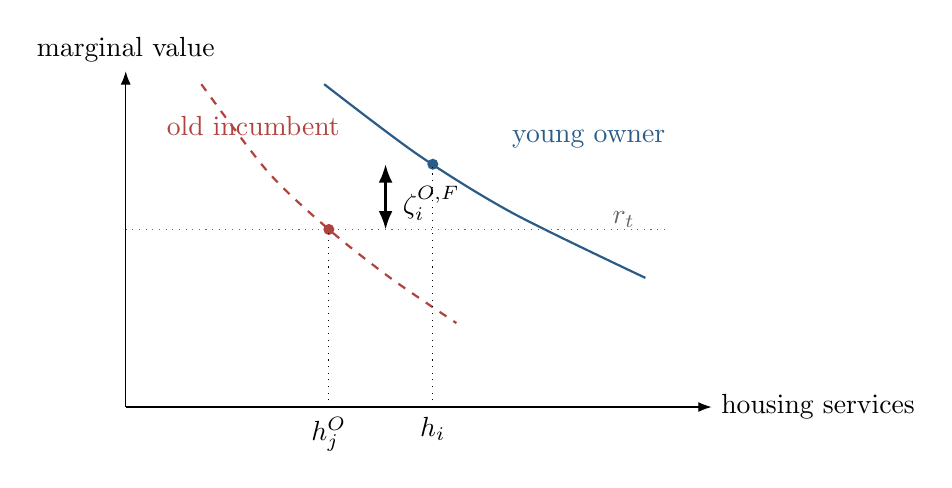
\begin{tikzpicture}[x=1.2cm,y=0.82cm,>=Latex]
  \draw[->] (0,0) -- (6.2,0) node[right] {housing services};
  \draw[->] (0,0) -- (0,5.2) node[above] {marginal value};
  \draw[oldblue,thick] plot[smooth] coordinates
    {(2.1,5.0) (3.1,3.9) (4.1,3.0) (5.5,2.0)};
  \draw[newred,thick,dashed] plot[smooth] coordinates
    {(0.8,5.0) (1.5,3.65) (2.15,2.75) (2.8,2.0) (3.5,1.3)};
  \draw[dotted,midgray] (0,2.75) -- (5.7,2.75);
  \node[right,midgray] at (5.05,2.9) {$r_t$};
  \fill[oldblue] (3.25,3.76) circle (2pt);
  \fill[newred] (2.15,2.75) circle (2pt);
  \draw[dotted] (3.25,0) -- (3.25,3.76);
  \draw[dotted] (2.15,0) -- (2.15,2.75);
  \draw[<->,thick] (2.75,2.75) -- (2.75,3.76);
  \node[right] at (2.83,3.15) {$\zeta_i^{O,F}$};
  \node[oldblue] at (4.9,4.15) {young owner};
  \node[newred] at (1.35,4.35) {old incumbent};
  \node[below] at (3.25,0) {$h_i$};
  \node[below] at (2.15,0) {$h_j^O$};
\end{tikzpicture}
\caption{In steady state, a constrained young owner values a marginal unit
above the common user cost, while an unconstrained incumbent values it at that
cost. The vertical distance is the financing component of the reallocation
surplus.}
\label{fig:reallocation}
\end{figure}

The reallocation result and the fertility response are distinct. Let
$A=1+\gamma+\omega_B$ and $k=\beta A$. With interior saving and old choices,
substituting the old allocation and the saving Euler equation into either young
problem gives the lifetime resource identity:
\begin{equation}
 (1+k)c+\chi n+r_t^m h=\mathcal W_t,
 \qquad
 \mathcal W_t=y_i+b_i+T_t+qT_{t+1}.
 \label{eq:lifetime_budget}
\end{equation}
Suppose an access constraint fixes the household's housing at $\widehat h$ while
fertility remains interior. Holding $\mathcal W_t$ and prices fixed, implicitly
differentiating the fertility condition yields:
\begin{equation}
 \frac{\dd n}{\dd \widehat h}
 =\frac{
 \dfrac{\alpha\kappa}{(\widehat h-\kappa n)^2}
 -\dfrac{(1+k)\chi r_t^m}
 {(\mathcal W_t-r_t^m\widehat h-\chi n)^2}}
 {\dfrac{\vartheta_t}{n^2}
 +\dfrac{(1+k)\chi^2}
 {(\mathcal W_t-r_t^m\widehat h-\chi n)^2}
 +\dfrac{\alpha\kappa^2}{(\widehat h-\kappa n)^2}}.
 \label{eq:fertility_cap_derivative}
\end{equation}
The first term in the numerator is the value of additional family space; the
second is the consumption cost of occupying more housing. Equation
\eqref{eq:housing_foc} implies
$[\mathcal W_t-r_t^m\widehat h-\chi n]/[\widehat h-\kappa n]
=(1+k)(r_t^m+\zeta_t^m)/\alpha$. Since $\zeta_t^m\geq0$, a sufficient
condition for greater housing access to raise fertility is:
\begin{equation}
 \chi\leq\frac{(1+k)\kappa r_t^m}{\alpha}.
 \label{eq:fertility_sufficient_condition}
\end{equation}
Under this condition, an institution that reaches a positive financing gap and
increases the household's housing both improves the conditional allocation and
raises fertility among the constrained households it directly affects.
General-equilibrium prices, rebates, and cohort sizes then propagate that
response through
equations~\eqref{eq:cohort_and_housing}--\eqref{eq:government_budget}.

\end{document}
